\documentclass[a4paper,12pt]{article} 


\usepackage[T2A]{fontenc}			
\usepackage[utf8]{inputenc}			
\usepackage[english,russian]{babel}	

\usepackage{graphicx, scalerel}    
\usepackage{wrapfig}               
\usepackage[14pt]{extsizes}        
\usepackage[warn]{mathtext}       
\usepackage{indentfirst}      
\usepackage[margin = 25mm]{geometry}
\usepackage[table,xcdraw]{xcolor} 
\usepackage{amsmath,amsfonts,amssymb,amsthm,mathtools}
\usepackage{wasysym}                
\usepackage{upgreek}                
\usepackage{caption}
\usepackage{multirow}
\captionsetup{labelsep=period}
\usepackage[font=small,labelfont=bf]{caption}
\usepackage{gensymb}
\usepackage{icomma}

\usepackage[unicode, pdftex]{hyperref}
\usepackage{tikz}
\usetikzlibrary{positioning}
\usepackage{fancyhdr}
\pagestyle{fancy}
\setlength\fboxsep{3pt} % Отступ рамки \fbox{} от рисунка
\setlength\fboxrule{1pt} % Толщина линий рамки \fbox{}
\usepackage{tocloft}
\newcommand{\tocsection}[1]{\section*{#1} \addcontentsline{toc}{section}{#1}}
\renewcommand{\cftsecleader}{\cftdotfill{\cftdotsep}}
\def\fillandplacepagenumber{%
	\par\pagestyle{empty}%
	\vbox to 0pt{\vss}\vfill
	\vbox to 0pt{\baselineskip0pt
		\hbox to\linewidth{\hss}%
		\baselineskip\footskip
		\hbox to\linewidth{%
			\hfil\thepage\hfil}\vss}}
		

\begin{document}
	\newcommand{\HRule}{\rule{\linewidth}{0.7mm}} % Defines a new command for the horizontal lines, change thickness here

\begin{center}
	\large\textbf{Московский Физико-Технический Институт}\\
	\large\textbf{(государственный университет)}
	
	\vfill
	
	
	
	\Large Лабораторная работа 5.1.2
	%----------------------------------------------------------------------------------------
	%	TITLE SECTION
	%----------------------------------------------------------------------------------------
	
	\HRule
	\\[0.4cm]
	{ \huge \bfseries Исследование эффекта Комптона}
	\\[0.4cm] % Title of your document
	\HRule
	\\[0.5cm]
	
	\ \\
	\textbf{\large Автор:} \\	
	\large Овсянников Михаил Б01-008\\
	\vfill
	\hspace*{-0.8 cm}
\includegraphics[width=100 pt]{./Include/frkt_logo.pdf}\\
	\large Долгопрудный, 2022
\end{center}

\thispagestyle{empty}

\newpage
\setcounter{page}{2}
\fancyfoot[c]{\thepage}
\fancyhead[L] {Лабораторная работа 5.1.2}
\fancyhead[R] {Исследование эффекта Комптона}

	\newpage
	
	\tableofcontents
	
	
	
	\newpage
	\textbf{Цель работы:} При помощи модели абсолютно черного тела (АЧТ) провести измерения температуры оптическим пирометром с исчезающей нитью и термопарой, исследовать излучение накаленных тел с различной испускательной способностью, определить постоянные Планка и Стефана–Больцмана.
	
	
	\tocsection{Теоретические сведения}
	
	Для измерения температуры разогретых тел, удаленных от наблюдателя, применяют методы оптической пирометрии, основанные на использовании зависимости испускательной способности исследуемого тела от температуры. Различают три температуры, функционально связанные с истинной термодинамической температурой и излучательной способностью тела: радиационную $T_\text{рад}$, цветовую $T_\text{цв}$ и яркостную $T_\text{ярк}$.

	
	Под радиационной (энергетической) температурой понимают температуру абсолютно черного тела, при которой его интегральная испускательная способность одинакова с интегральной испускательной способностью исследуемого тела.

	Под цветовой температурой исследуемого тела понимают температуру абсолютно черного тела, при которой отношение их спектральных испускательных способностей для двух заданных длин волн одинаково.
	
	Под яркостной температурой понимают температуру абсолютно черного тела, при которой его спектральная испускательная способность равна спектральной испускательной способности исследуемого тела при той же длине волны. Именно эту температуру мы будем измерять в данной работе.

	
	Измерение яркостной температуры раскаленного тела производится при помощи оптического пирометра с исчезающей нитью, основанного на визуальном сравнении яркости раскаленной нити с яркостью изображения исследуемого тела. 
	
	Оптический пирометр представляет собой зрительную трубу, внутри которой имеется накаливаемая нить, расположенная в плоскости изображения исследуемого раскаленного тела, а также темно-красный светофильтр. Через окуляр одновременно наблюдается изображение исследуемого тела и раскаленной нити.
	
	Если в том узком спектральном интервале, который пропускается светофильтром, яркость нити меньше яркости раскаленного тела, то нить видится темной полоской на светлом фоне, и наоборот. При совпадении яркостей нить перестает быть видимой на фоне изображения раскаленного тела. Регулировка яркости нити осуществляется изменением тока, протекающего через нее.
	
	\begin{figure}[h!]
		\centering
		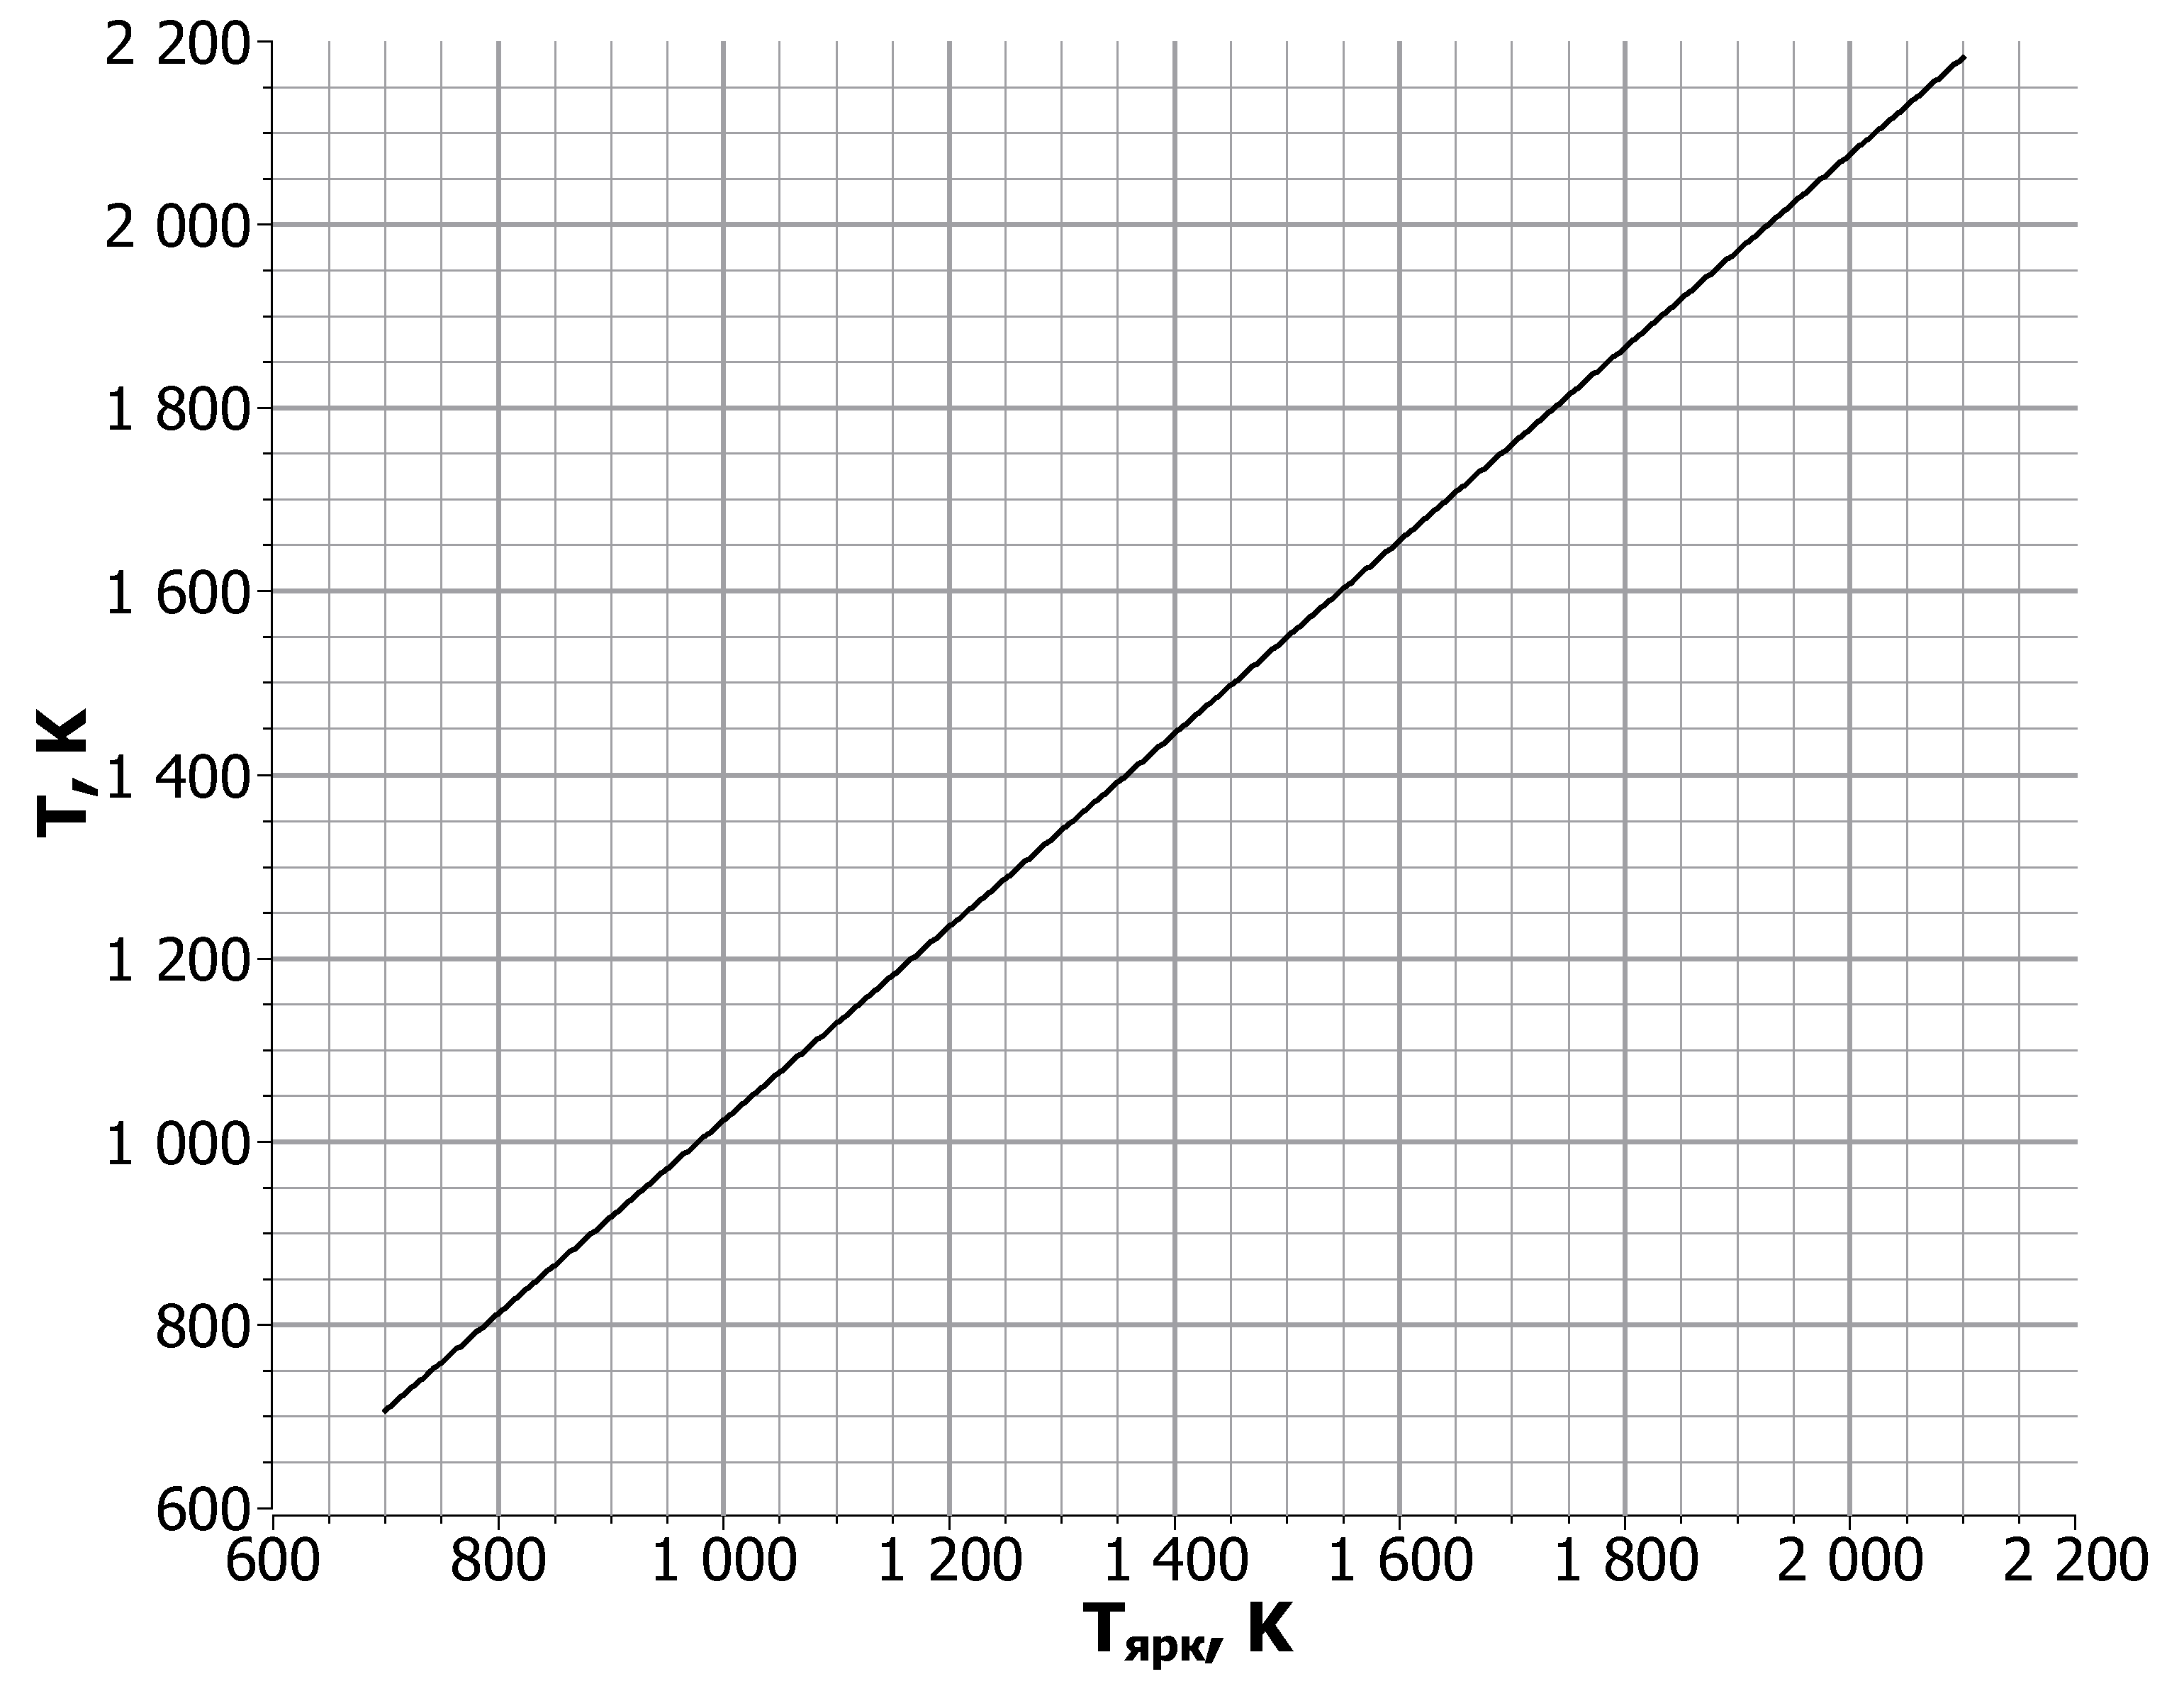
\includegraphics[width=\linewidth]{./Pictures/T(T_bright).pdf}
		\caption{График зависимости $T = f(T_\text{ярк})$ для вольфрама}
		\label{Stefan_Boltz_T(T_bright)}
	\end{figure}
	
	
	Если предположить, что нить излучает как серое тело, то выражение
	(Рис. \ref{Stefan_Boltz_T(T_bright)}) можно записать в виде
	\begin{equation}
		W = \varepsilon_T S\sigma T^4.
		\label{Stefan_Boltz_W(E_T_and_T)}
	\end{equation}

 	Значения коэффициента излучения $\varepsilon_T$ при различных температурах приведены в таблице \ref{Stefan_Boltz_E_T(T)}.

 	\begin{table}[h!]
 		\centering
 		\resizebox{\columnwidth}{!}{%
 			\begin{tabular}{|c|c|c|c|c|c|c|c|c|c|c|c|c|c|}
 				\hline
 				$T$, K          & 800   & 900   & 1000  & 1100  & 1200  & 1300  & 1400  & 1500  & 1600  & 1700  & 1800  & 1900  & 2000  \\ \hline
 				$\varepsilon_T$ & 0,067 & 0,081 & 0,105 & 0,119 & 0,133 & 0,144 & 0,164 & 0,179 & 0,195 & 0,209 & 0,223 & 0,236 & 0,249 \\ \hline
 			\end{tabular}%
 		}
 	\caption{Поправочные коэффициенты излучения для вольфрама}
 	\label{Stefan_Boltz_E_T(T)}
 	\end{table}
 
 	Измерив температуру вольфрамовой нити в зависимости от подводимой мощности, можно убедиться в справедливости закона Стефана–Больцмана применительно к серому телу (в данном случае к вольфраму). Из формулы \eqref{Stefan_Boltz_W(E_T_and_T)} можно определить также и величину постоянной $\sigma$ в законе Стефана–Больцмана.


	
	\newpage
	\tocsection{Экспериментальная установка}
	\begin{figure}[h!]
		\centering
		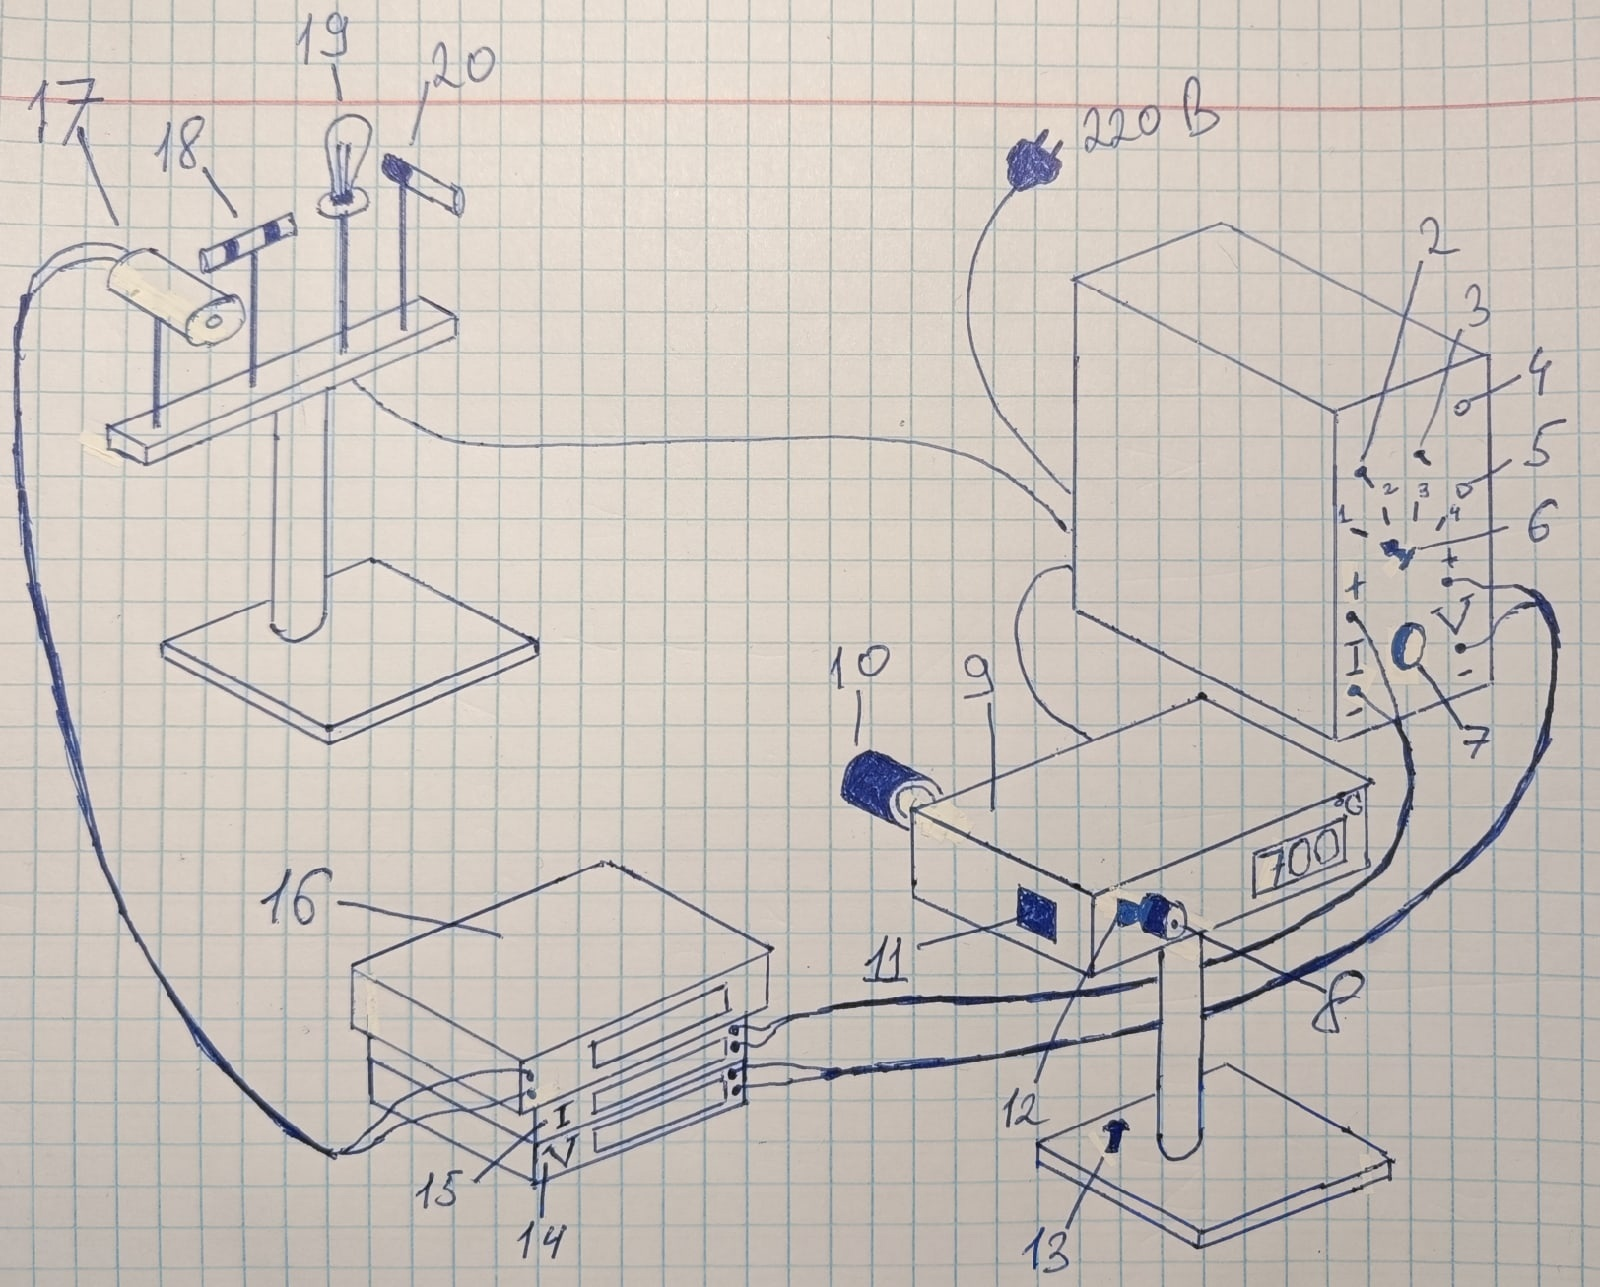
\includegraphics[width=\linewidth]{Pictures/Scheme.jpg}
		\caption{Схема экспериментальной установки}
		\label{Stefan_Boltz_Scheme}
	\end{figure}

	1 — блок питания; 2 — тумблер включения питания пирометра и образцов; 3 — тумблер нагрева нити пирометра: «Быстро» — вверх, «Медленно» — вниз; 4 — кнопка «Нагрев нити»; 5 — кнопка «охлаждение нити»; 6 — тумблер переключения образцов; 7 — регулятор мощности нагрева образцов; 8 — окуляр пирометра; 9 — корпус пирометра; 10 — объектив пирометра; 11 — переключение диапазонов: 700–1200$^\circ$C — вниз, 1200–2000$^\circ$C — вверх; 12 — ручка перемещения красного светофильтра; 13 — регулировочный винт; 14 — вольтметр (напряжение на лампе накаливания); 15 — амперметр (ток через образцы); 16 — вольтметр в цепи термопары; 17 — модель АЧТ; 18 — трубка с кольцами из материалов с разной излучательной способностью; 19 — лампа накаливания; 20 — неоновая лампочка.
	
	Экспериментальная установка (Рис. \ref{Stefan_Boltz_Scheme}) состоит из оптического пирометра 9, модели абсолютно черного тела (АЧТ), трех исследуемых образцов (18, 19, 20), блока питания (1) и цифровых вольтметров В7-22А и В7-38.
	
	Пирометр 9 с исчезающей нитью включает в себя объектив 10, окуляр 8, монохроматический (красный) светофильтр 4, позволяющий рассматривать в лучах красного цвета нить пирометра на фоне изображения накаленного исследуемого тела. Перемещение светофильтра осуществляется сектором 12.
	
	Модель АЧТ представляет собой керамическую трубку диаметром 3 мм и длиной 50 мм, закрытую с одного конца и окруженную для теплоизоляции внешним кожухом. Нагрев трубки осуществляется намотанной на ней нихромовой спиралью, питаемой от источника тока. Полость трубки и особенно ее дно излучают практически как абсолютно черное тело. Температура модели АЧТ измеряется хромель-алюмелевой термопарой, один спай которой вмонтирован в дно трубки, а другой находится при комнатной температуре на клемме цифрового вольтметра В7-38, измеряющего ЭДС термопары.

	
	В работе исследуются три образца. Один образец выполнен в виде керамической трубки с набором колец из различных материалов, нагреваемой изнутри нихромовой спиралью. Материалы колец имеют различную испускательную способность. Спираль подключается к источнику питания 1 с помощью переключателя 6 (положение 2) и может нагревать трубку до температуры около 1100 $^\circ$C. Термодинамическая температура колец практически одинакова и равна температуре трубки.

	
	Другой исследуемый образец — вольфрамовая нить электрической лампочки. Она питается от источника 1, когда переключатель 6 находится в положении 3. Сила тока через вольфрамовую нить измеряется с помощью прибора В7-22А (15). Падение напряжения на самой нити измеряется непосредственно вольтметром В7-22А (16). Таким образом, зная показания обоих приборов, можно определить мощность, потребляемую нитью лампочки.
	
	Источник питания 1, используемый в работе, снабжен устройством, отключающим в случае перегрузки прибор от потребителя, в этот момент загорается сигнальная лампочка «перегрузка» на передней панели прибора. Если это произойдет, то надо отключить питание прибора от сети 220 В и уменьшить напряжение на его выходе, а затем повторно включить источник питания.

	
	
	
	\newpage
	\tocsection{Ход работы}
	\begin{center}
		\textbf{I. Изучение работы оптического пирометра}
	\end{center}
	\begin{enumerate}
		\item Выведем оба светофильтра пирометра (серый и красный) с помощью переключателя 11 и сектора 12.
		
		\item Подключим питание пирометра и образцов с помощью тумблера 2 к сети 220 В.
		
		\item Нажмем кнопку 4 и, удерживая ее, доведем показания пирометра, а, следовательно, и температуру его нити до 900 -- 950 $^\circ$C. Направим пирометр на модель АЧТ. Переключатель 6 поставим в положение 1 (АЧТ), подав тем самым питание на нагревательную спираль модели АЧТ. Повернем ручку 7 регулятора мощности нагрева по часовой стрелке до упора. Через 10–15 минут дно модели АЧТ нагреется до красного каления.

		
		Перемещением объектива 10 пирометра добьемся четкого изображения поверхности дна модели АЧТ.
		
		\item Введем поворотом сектора 12 красный светофильтр пирометра.
		
		\item Нажмем и будем удерживать кнопку 4 или 5, увеличивая или уменьшая ток через нить пирометра, добьемся исчезновения нити на фоне изображения раскаленной поверхности дна модели АЧТ. Опыт повторим несколько раз, подходя поочередно от меньшей яркости, когда нить кажется темной на фоне дня АЧТ, и от большей яркости, когда нить кажется более светлой, чем дно АЧТ.

		
		\item Определим по шкале пирометра значение яркостной температуры модели АЧТ. Одновременно следует измерить температуру модели АЧТ при помощи хромель-алюмелевой термопары и цифрового вольтметра 16. Результаты поместим в таблицу \ref{Stefan_Boltz_Pyro_Pair}.
		
	
		\begin{table}[h!]
			\centering
			\resizebox{\columnwidth}{!}{%
				\begin{tabular}{|c|c|}
					\hline
					Показания пирометра $T_\text{ярк}$, K & Показания термопары $T_\text{ярк}$, K \\ \hline
					1243                                & \multirow{2}{*}{1232}                \\ \cline{1-1}
					1244                                &                                      \\ \hline
				\end{tabular}%
			}
			\caption{Яркостная температура АЧТ}
			\label{Stefan_Boltz_Pyro_Pair}
		\end{table}
	
		Как видим, результаты достаточно близки друг к другу, даже почти совпадают. Погрешность составляет $\sim 1\%$. Следовательно, пирометр работает исправно.
	\end{enumerate}

	\begin{center}
		\textbf{II. Измерение яркостной температуры накаленных тел}
	\end{center}

	\begin{enumerate}
		\item Этот эксперимент предполагает показать, что различные тела, накаленные до одинаковой термодинамической температуры, имеют различную яркостную температуру.
		
		\item Направим пирометр на поверхность керамической трубки с кольцами из различных материалов. Переключатель 6 поставим в положение 2 «Кольца». Так же, как и в пункте I, установив регулятор мощности нагрева 7 на максимум, нагреем трубку до темно-красного каления.
		
		\item Измерим яркостную температуру поверхности трубки и каждого из колец. Результаты заносим в таблицу \ref{Stefan_Boltz_Tube_Rings}.
		
		
		\begin{table}[h!]
			\centering

			\begin{tabular}{|c|c|}
				\hline
				Тело          & Яркостная температура $T_\text{ярк}$, K \\ \hline
				Трубка        & 1188                                    \\ \hline
				Левое кольцо  & 1123                                    \\ \hline
				Правое кольцо & 1113                                    \\ \hline
			\end{tabular}
			\caption{Яркостная температура разных тел}
			\label{Stefan_Boltz_Tube_Rings}
		\end{table}
	
		Как видим, яркостные температуры для этих тел различны. Объясняется это тем, что каждое из этих тел лишь на какую-то долю можно считать АЧТ, причем у тел эти доли разные.
	\end{enumerate}

	\begin{center}
		\textbf{III. Проверка закона Стефана–Больцмана}
	\end{center}

	\begin{enumerate}
		\item Направим пирометр на нить лампы накаливания. Поставим переключатель 6 в положение 3 (<<Лампа>>).
		
		\item Постепенно увеличивая при помощи ручки «7» накал нити лампы, начиная со слабого темно-красного накала вплоть до 1900 $^\circ$C, будем измерять пирометром яркостную температуру нити через каждые 100 $^\circ$C. При каждом измерении температуры будем записывать также величину тока и падения напряжения на нити лампы.
Данные занесем в таблицу \ref{Stefan_Boltz_W(T)}.
		
		\item Для каждого значения измеренной яркостной температуры найдем термодинамическую температуру вольфрамовой нити лампы, пользуясь графиком (\ref{Stefan_Boltz_T(T_bright)}): $T = f_1(T_\text{ярк})$. $T$ — абсолютная температура. Вычислим для каждого значения термодинамической температуры мощность, потребляемую нитью лампы. Вычисления запишем в таблицу \ref{Stefan_Boltz_W(T)}. Также построим таблицу для значений с их погрешностями \ref{Stefan_Boltz_W(T)_Flaws}.
		
		Для лучшего визуального анализа построим график зависимости $W = f_2(T)$.
		\begin{figure}[h!]
			\centering
			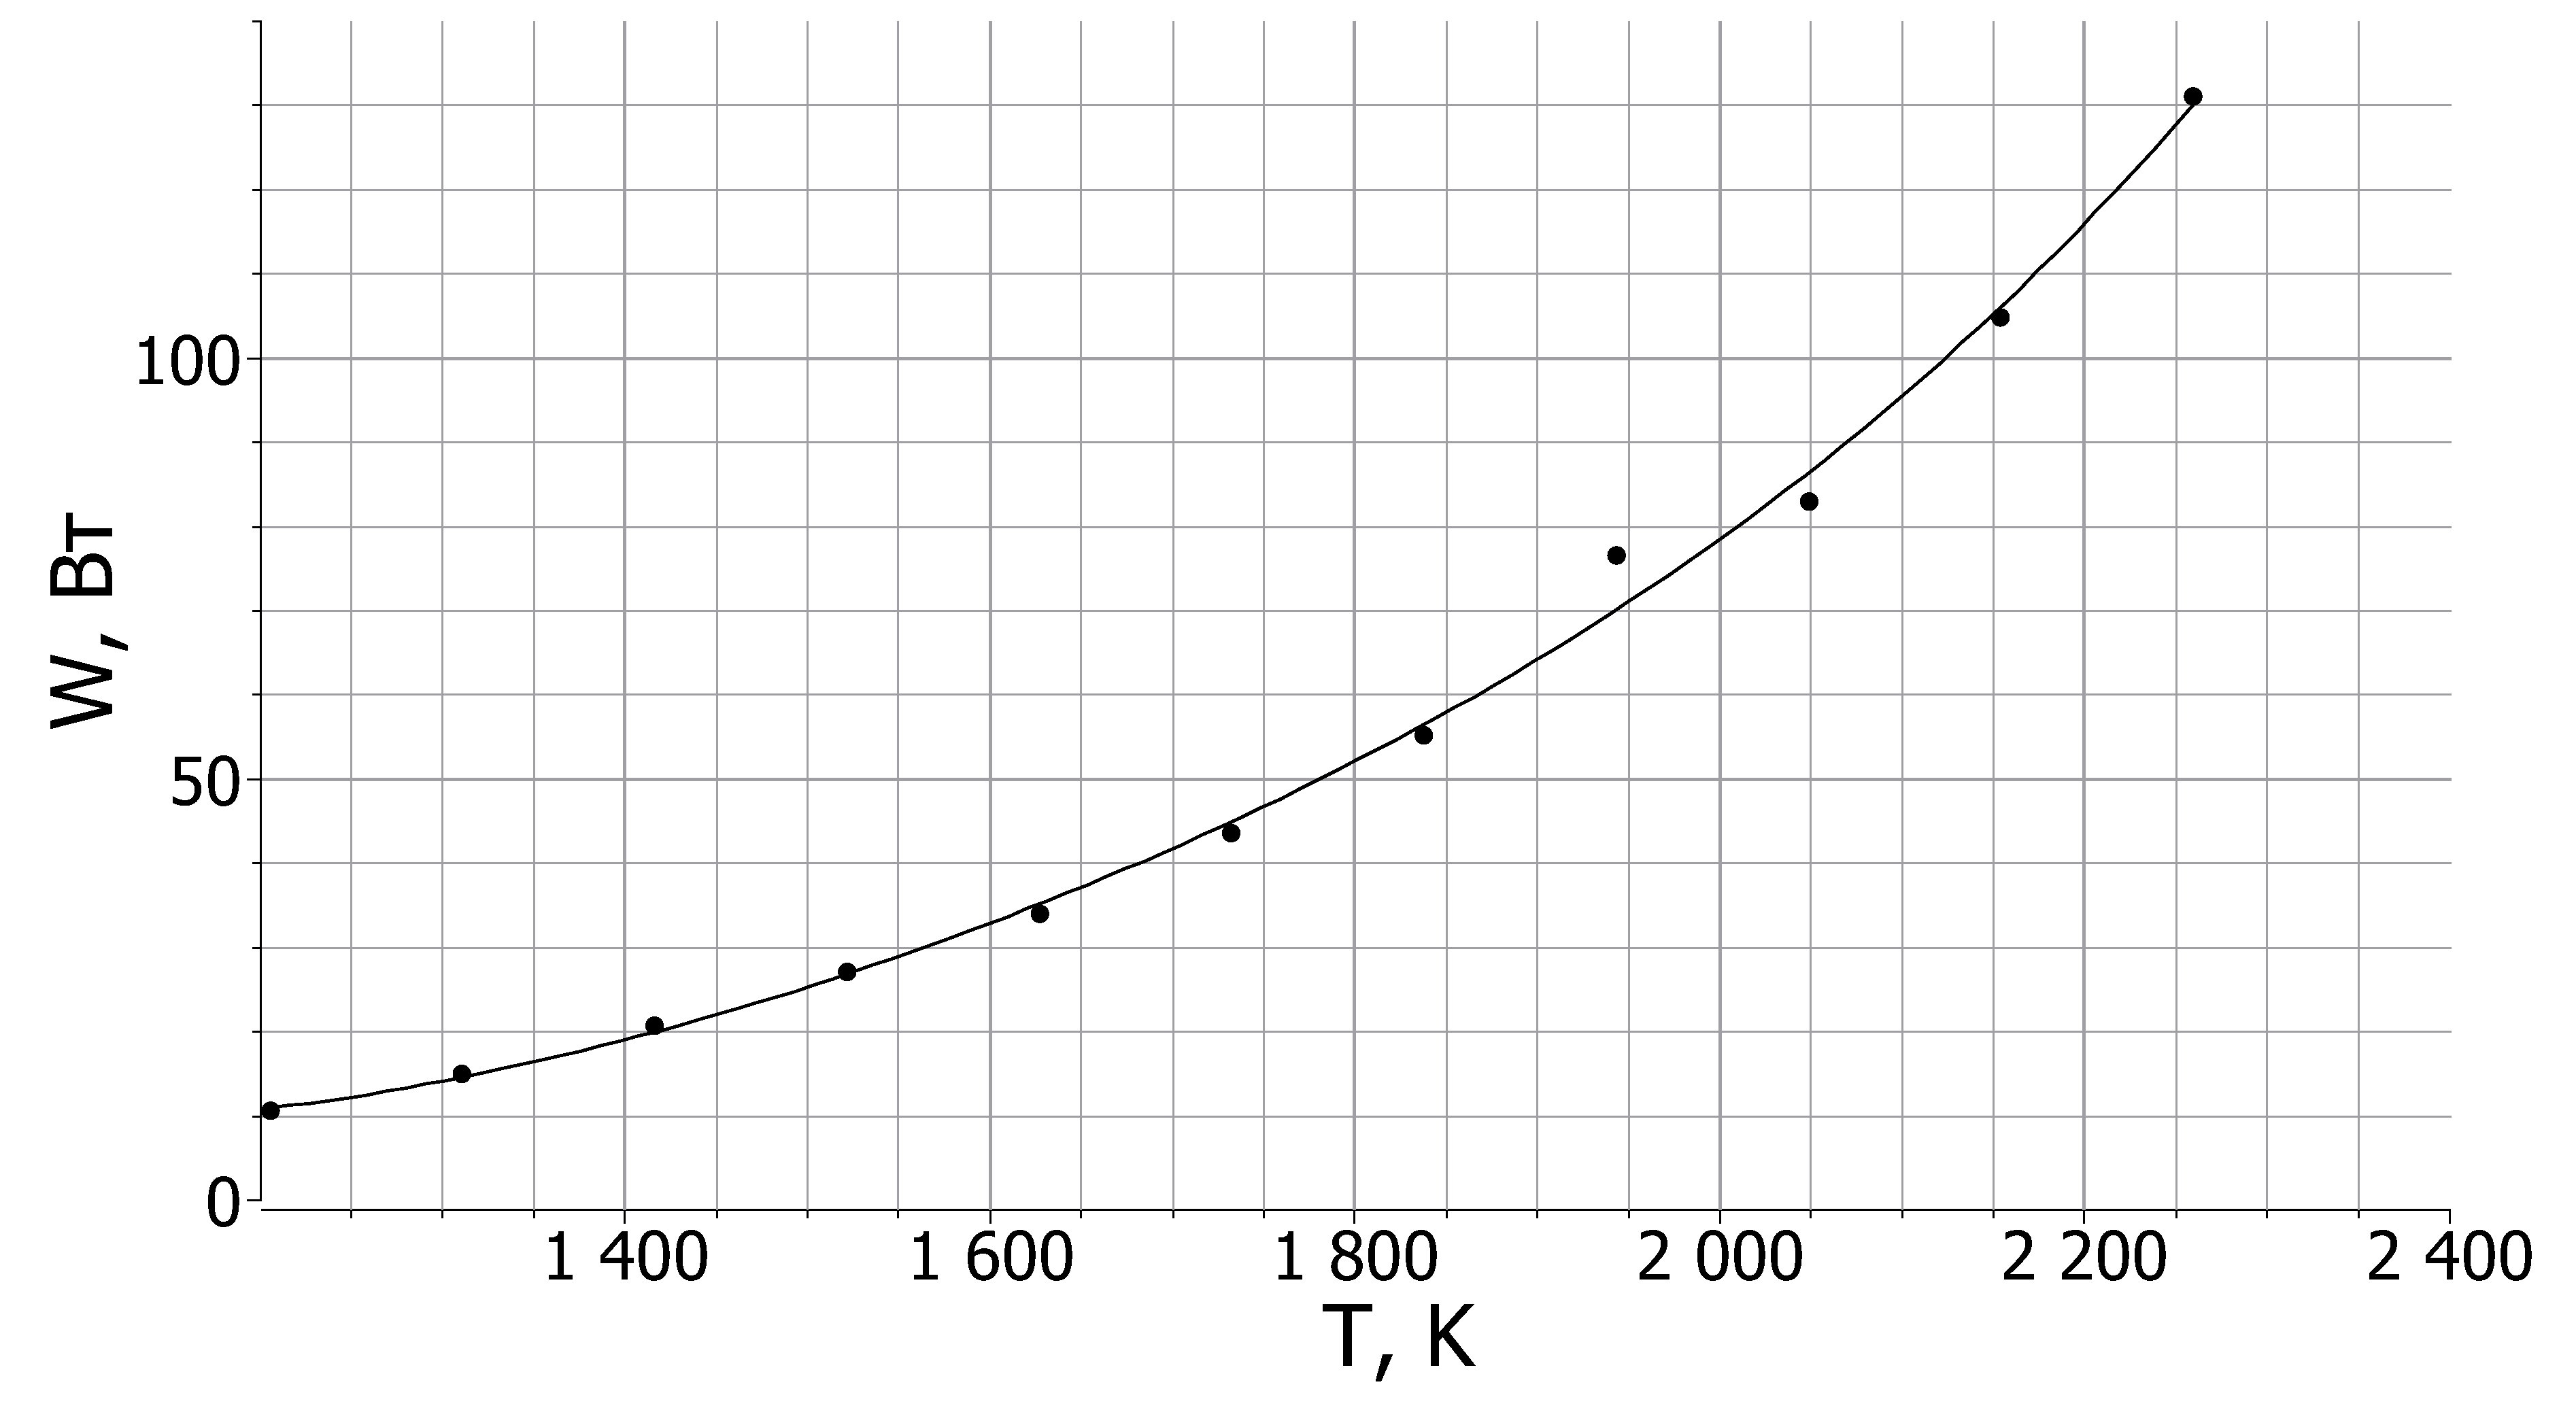
\includegraphics[width=\linewidth]{Pictures/W(T).pdf}
			\caption{График зависимости $W(T)$}
		\end{figure}
		

		\begin{table}[h!]
			\centering
				\begin{tabular}{|r|r|r|r|r|r|}
					\hline
					\multicolumn{1}{|c|}{$t$, $^\circ$C} & \multicolumn{1}{c|}{$T_\text{ярк}$, K} & \multicolumn{1}{c|}{$T$, K} & \multicolumn{1}{c|}{$I$, А} & \multicolumn{1}{c|}{$V$, В} & \multicolumn{1}{c|}{$W$, Вт} \\ \hline
					900                                  & 1173                                   & 1205                        & 0,637                       & 16,51                       & 10,52                        \\ \hline
					1000                                 & 1273                                   & 1311                        & 0,703                       & 21,31                       & 14,98                        \\ \hline
					1100                                 & 1373                                   & 1416                        & 0,772                       & 26,81                       & 20,70                        \\ \hline
					1200                                 & 1473                                   & 1522                        & 0,837                       & 32,35                       & 27,08                        \\ \hline
					1300                                 & 1573                                   & 1627                        & 0,900                       & 37,77                       & 33,99                        \\ \hline
					1400                                 & 1673                                   & 1732                        & 0,977                       & 44,62                       & 43,60                        \\ \hline
					1500                                 & 1773                                   & 1838                       & 1,057                       & 52,25                       & 55,23                        \\ \hline
					1600                                 & 1873                                   & 1943                        & 1,145                       & 66,89                       & 76,59                        \\ \hline
					1700                                 & 1973                                   & 2049                        & 1,215                       & 68,30                       & 82,98                        \\ \hline
					1800                                 & 2073                                   & 2154                        & 1,317                       & 79,60                       & 104,83                       \\ \hline
					1900                                 & 2173                                   & 2259                        & 1,426                       & 91,90                       & 131,05                       \\ \hline
				\end{tabular}
			\caption{Зависимость мощности от температуры}
			\label{Stefan_Boltz_W(T)}
		\end{table}
	
		\begin{landscape}
			\thispagestyle{empty}
			\begin{table}[h!]
				\centering
				\resizebox{\columnwidth}{!}{%
					\begin{tabular}{|r|r|r|r|r|r|r|r|r|r|r|r|r|r|r|r|}
						\hline
						$t$, $^\circ$C & $\sigma_t$ & $T_\text{ярк}$, K & $\sigma_{T_\text{ярк}}$, K & $T$, K & $\sigma_T$, K & $I$, А & $\sigma_I$, А & $V$, В & $\sigma_V$, В & $W$, Вт & $\sigma_W$, Вт & \multicolumn{1}{c|}{$\ln T$}  & $\sigma_{\ln T}$ & \multicolumn{1}{c|}{$\ln W$}  & $\sigma_{\ln W}$ \\ \hline
						900            & 1          & 1173              & 1                          & 120    & 1,054         & 0,637  & 0,001         & 16,51  & 0,01          & 10,52   & 0,02           & 7,094602 & 0,0009           & 2,352981 & 0,002            \\ \hline
						1000           & 1          & 1273              & 1                          & 1311   & 1,054         & 0,703  & 0,001         & 21,31  & 0,01          & 14,98   & 0,02           & 7,178425 & 0,0008           & 2,706778 & 0,002            \\ \hline
						1100           & 1          & 1373              & 1                          & 1416   & 1,054         & 0,772  & 0,001         & 26,81  & 0,01          & 20,70   & 0,03           & 7,255762 & 0,0008           & 3,030004 & 0,002            \\ \hline
						1200           & 1          & 1473              & 1                          & 1522   & 1,054         & 0,837  & 0,001         & 32,35  & 0,01          & 27,08   & 0,04           & 7,327545 & 0,0007           & 3,298683 & 0,002            \\ \hline
						1300           & 1          & 1573              & 1                          & 1627   & 1,054         & 0,900  & 0,001         & 37,77  & 0,01          & 33,99   & 0,04           & 7,394519 & 0,0007           & 3,526155 & 0,002            \\ \hline
						1400           & 1          & 1673              & 1                          & 1732   & 1,054         & 0,977  & 0,001         & 44,62  & 0,01          & 43,59   & 0,05           & 7,457287 & 0,0006           & 3,774914 & 0,001            \\ \hline
						1500           & 1          & 1773              & 1                          & 1838   & 1,054         & 1,057  & 0,001         & 52,25  & 0,01          & 55,23   & 0,06           & 7,516347 & 0,0006           & 4,011475 & 0,001            \\ \hline
						1600           & 1          & 1873              & 1                          & 1943   & 1,054         & 1,145  & 0,001         & 66,89  & 0,01          & 76,59   & 0,07           & 7,572113 & 0,0006           & 4,338454 & 0,001            \\ \hline
						1700           & 1          & 1973              & 1                          & 2049   & 1,054         & 1,215  & 0,001         & 68,30  & 0,01          & 82,98   & 0,07           & 7,624933 & 0,0006           & 4,418654 & 0,001            \\ \hline
						1800           & 1          & 2073              & 1                          & 2154   & 1,054         & 1,317  & 0,001         & 79,60  & 0,01          & 104,83  & 0,08           & 7,675101 & 0,0005           & 4,652371 & 0,001            \\ \hline
						1900           & 1          & 2173              & 1                          & 2259   & 1,054         & 1,426  & 0,001         & 91,90  & 0,01          & 131,05  & 0,10           & 7,722873 & 0,0005           & 4,875574 & 0,001            \\ \hline
					\end{tabular}%
				}
				\caption{Зависимость мощности от температуры вместе с погрешностями}
				\label{Stefan_Boltz_W(T)_Flaws}
			\end{table}
		\fillandplacepagenumber
		\end{landscape} 
	
 		\item Для проверки закона Стефана–Больцмана построим в логарифмическом масштабе график зависимости $W = \varepsilon_T B T^n$, т. е. функцию 
 		\begin{equation*}
 			\ln W = \ln (\varepsilon_T B) + n\ln T
 		\end{equation*}
 		\noindent и определим величину $n$ как тангенс угла наклона прямой.
 		
 		\begin{figure}[h!]
 			\centering
 			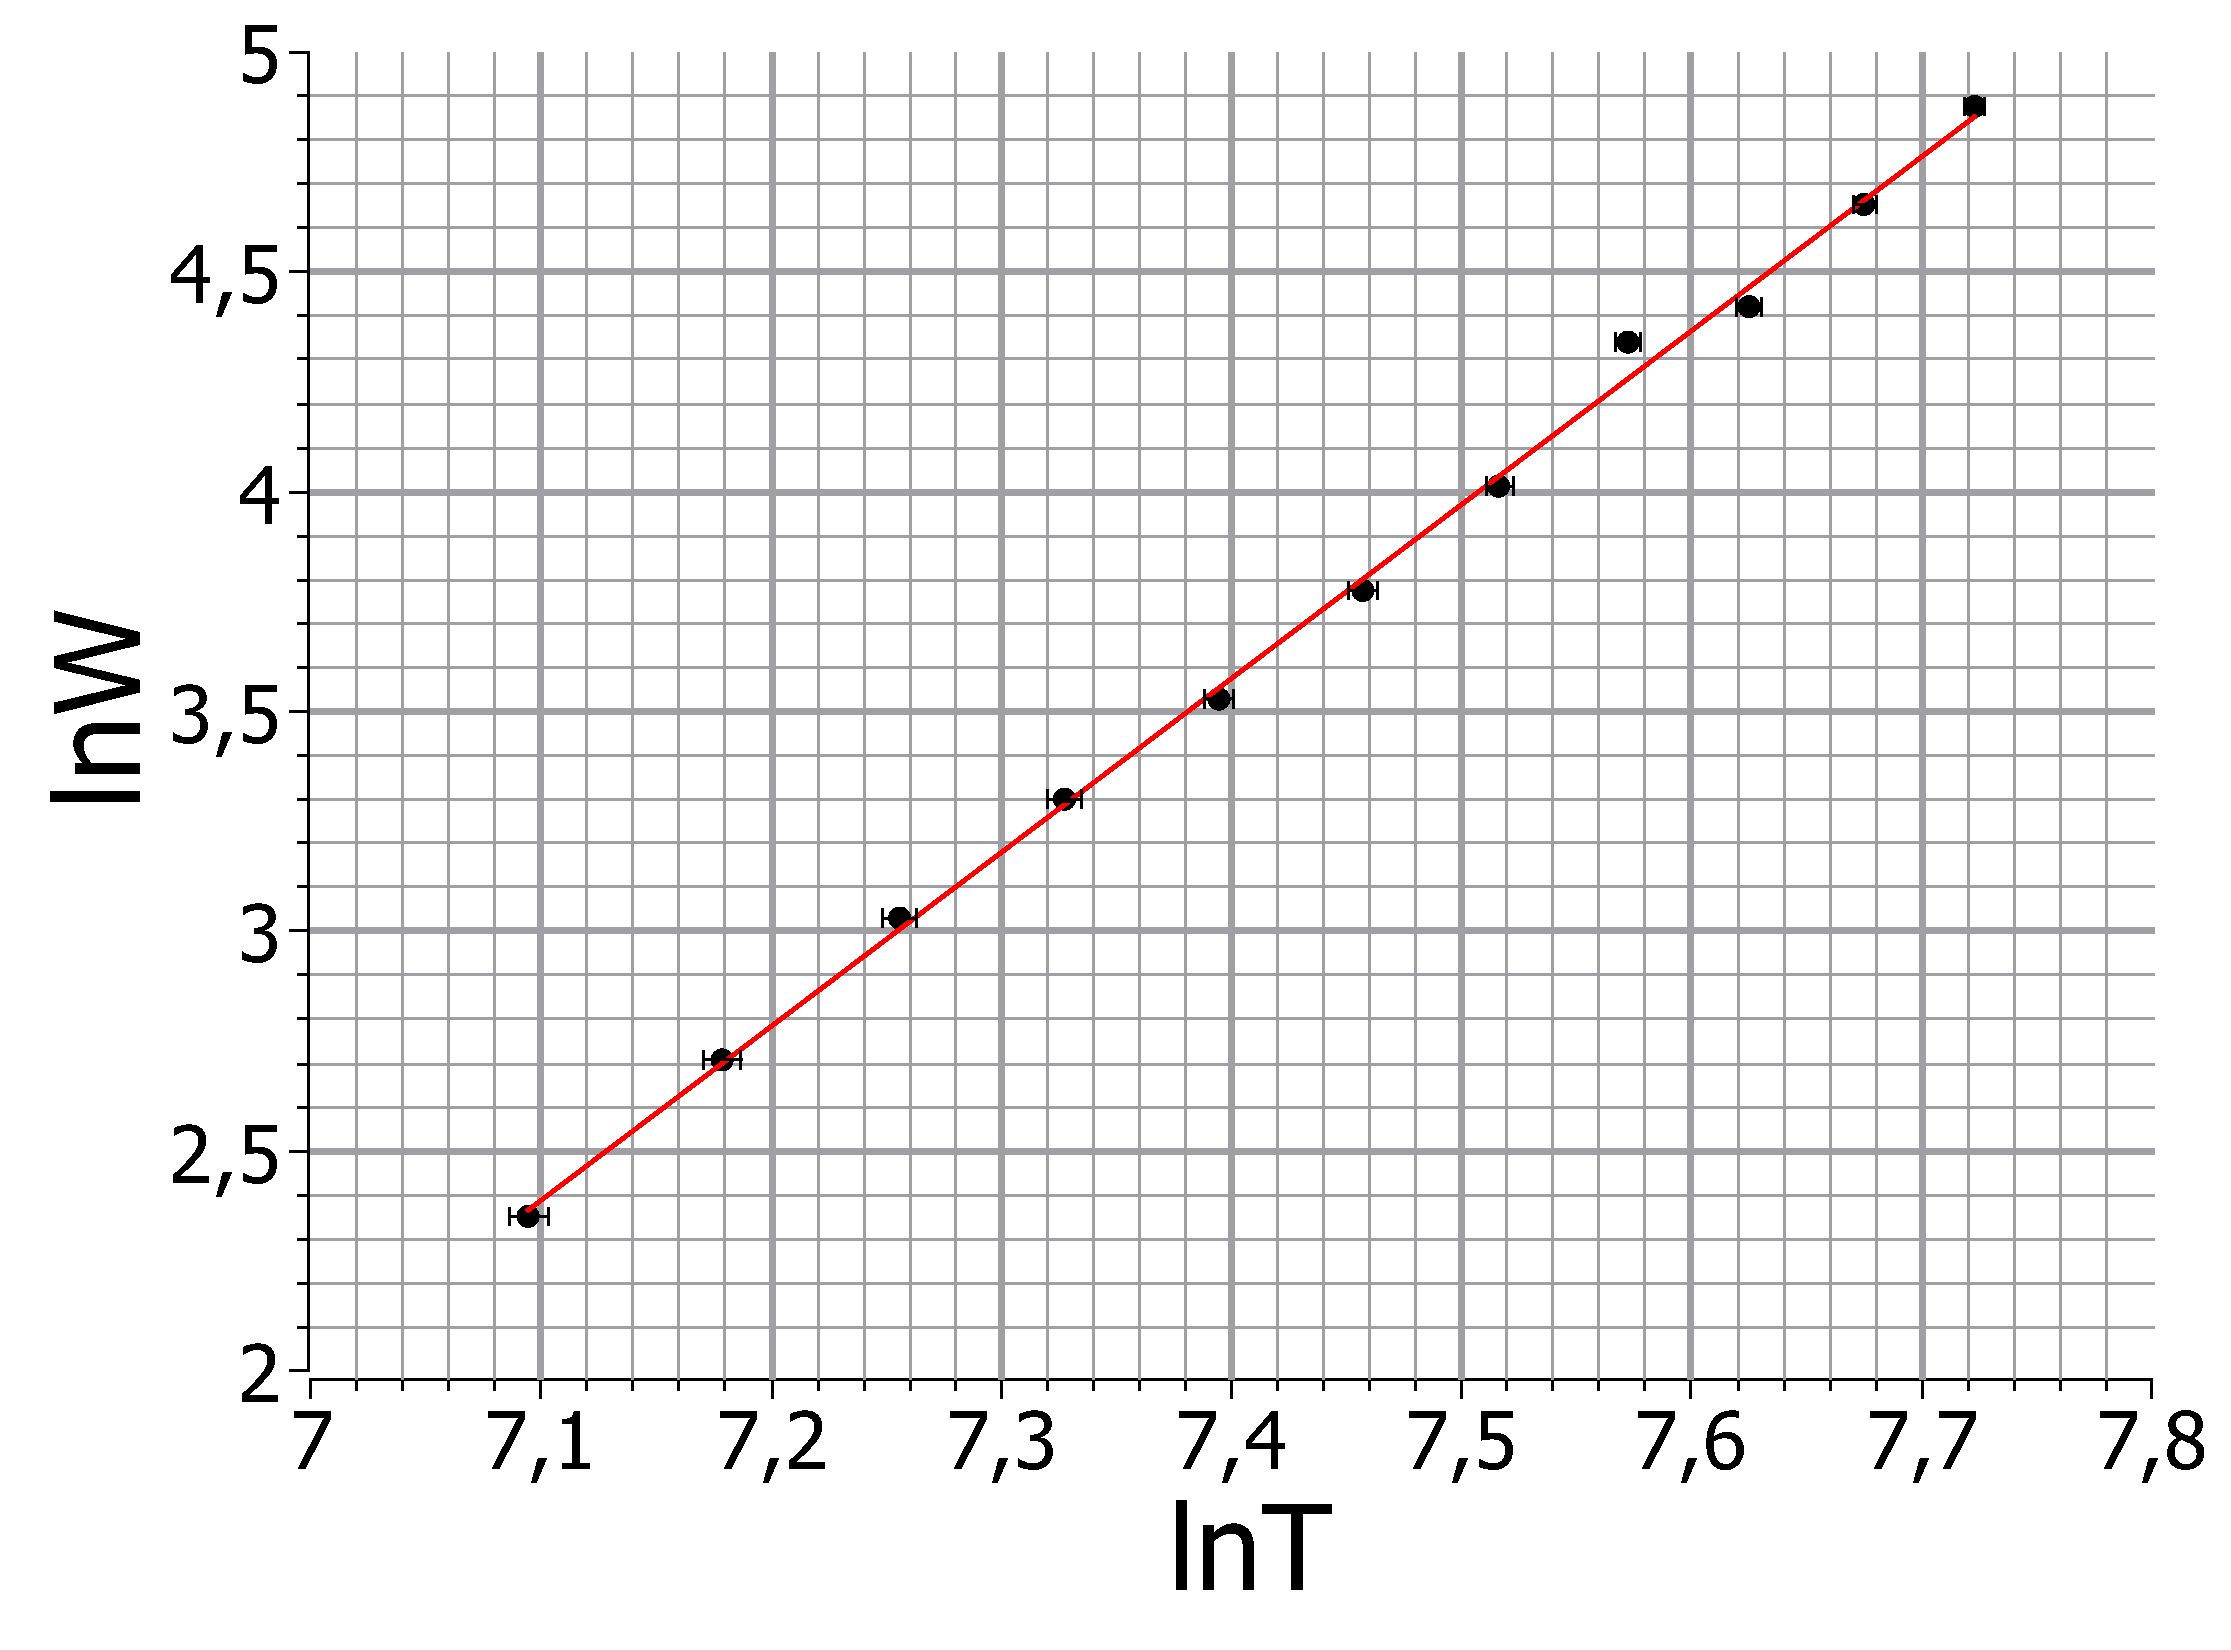
\includegraphics[width=\linewidth]{Pictures/lnW(lnT)2.pdf}
 			\caption{Зависимость $\ln W(\ln T)$}
 		\end{figure}
 	
 		Из графика мы получаем следующее:
 		\begin{itemize}
 			\item $n = (3,96 \pm 0,05)$. То есть очень близко к теоретическому $n = 4$ и в пределах погрешности даже совпадает с ним.
 			
 			\item $\ln (\varepsilon_T B) = (-25,7 \pm 0,4)$.
 		\end{itemize}
		
		
		\item Найдем величину постоянной Стефана–Больцмана по формуле
		\begin{equation*}
			\sigma = \frac{W}{\varepsilon_T S T^4}
		\end{equation*}
		\noindent для каждого значения $T$, превышающего $1700$ K. Расчеты приведены в таблице \ref{Stefan_Boltz_Sigma_Table}:
		
		\newpage
		\renewcommand{\arraystretch}{2.2}
		\begin{table}[h!]
			\centering
				\begin{tabular}{|r|r|}
					\hline
					$T$, K & \multicolumn{1}{c|}{$\sigma$, $\dfrac{\text{Вт}}{\text{м}^2 \cdot \text{K}^4}$} \\ \hline
					1732   & $(6,33 \pm 0,02) \cdot 10^{-7}$                                                 \\ \hline
					1838   & $(5,89 \pm 0,02) \cdot 10^{-7}$                                                 \\ \hline
					1943   & $(6,10 \pm 0,02) \cdot 10^{-7}$                                                 \\ \hline
					2049   & $(5,02 \pm 0,02) \cdot 10^{-7}$                                                 \\ \hline
					2154   & $(4,89 \pm 0,02) \cdot 10^{-7}$                                                 \\ \hline
					2259   & $(4,77 \pm 0,01) \cdot 10^{-7}$                                                 \\ \hline
				\end{tabular}
				\caption{Значения постоянной Стефана-Больцмана для разных температур}
				\label{Stefan_Boltz_Sigma_Table}
		\end{table}
	
		Как видим, все значения одного порядка. Однако они на порядок больше табличного значения $\sigma = 5,67 \cdot 10^{-8} \dfrac{\text{Вт}}{\text{м}^2 \cdot \text{K}^4}$.
		
		Общее значение из эксперимента $\sigma = (5,50 \pm 0,02) \cdot 10^{-7}$ $\dfrac{\text{Вт}}{\text{м}^2 \cdot \text{K}^4}$.
		
		
		\item По найденному значению $\sigma$ определим величину постоянной Планка $h$ по формуле:
		\begin{equation*}
			h = \sqrt[3]{\frac{2\pi^5 k_\text{Б}^4}{15\sigma c^2}}
		\end{equation*}
	
		Отсюда выходит:
		\begin{equation*}
			h = (3,104 \pm 0,004) \cdot 10^{-34} \text{ Дж}\cdot\text{с}
		\end{equation*}
	
		Значение совпадает по порядку с табличным $h = 6,626 \cdot 10^{-34}  \text{ Дж}\cdot\text{с}$, отличие в 2 раза.
	\end{enumerate}


	\begin{center}
		\textbf{IV. Измерение «яркостной температуры» неоновой лампочки}
	\end{center}
	Направим пирометр на неоновую лампочку. Поставим переключатель 6 в положение 4 («Неоновая лампочка») и измерим пирометром «яркостную температуру» неоновой лампочки. $T_\text{ярк} = 1295$ K. 
	
	Дотронувшись до лампочки рукой, убедимся, что термодинамическая температура лампочки не соответствует измеренной «яркостной температуре» нагретого тела.
Лампочка чуть тепла.
	
	
	\tocsection{Вывод}
	В данной работе мы провели исследование излучения накаленных тел с различной испускательной способностью. Мы убедились, что яркостная температура меньше термодинамической, причем у разных тел при одинаковой термодинамической разная яркостная. Вдобавок, мы смогли экспериментально оценить значение постоянной Стефана--Больцмана $\\\sigma = (5,50 \pm 0,02) \cdot 10^{-7}$ $\frac{\text{Вт}}{\text{м}^2 \cdot \text{K}^4}$. Отличие от табличного значения на порядок. Также, рассчитали постоянную Планка $h = (3,104 \pm 0,004) \cdot 10^{-34} \text{ Дж}\cdot\text{с}$. Это значение отличается от табличного в 2 раза (что и происходит, поскольку $\sigma$ отличается от табличного на порядок). Такие большие отличия обусловлены несовершенством методики измерения.
		
\end{document}